\documentclass[tikz,border=6pt]{standalone}
\usepackage[utf8]{inputenc}
\usepackage{xcolor}
\usepackage{amsmath}
\usetikzlibrary{arrows.meta,calc,positioning,fit}
\renewcommand{\familydefault}{\sfdefault}

\definecolor{medBlue}    {HTML}{4A86B8}
\definecolor{constGray}  {HTML}{9E9E9E}
\definecolor{loss1}      {HTML}{F1D897}
\definecolor{panelGray}  {HTML}{CFCFCF}

\tikzset{
  font=\sffamily\footnotesize,
  arrow/.style={-{Latex[length=2.2mm,width=1.7mm]},draw=black,line width=1.0pt},
  panel/.style={rounded corners=8pt,draw=panelGray,dashed,line width=1.2pt,fill=white},
  model/.style={rectangle,rounded corners=3pt,draw=none,fill=medBlue,text=white,
    minimum width=4.2cm,minimum height=1.6cm,align=center,inner xsep=6pt,font=\bfseries\footnotesize},
  constmodel/.style={rectangle,rounded corners=3pt,draw=none,fill=constGray,text=white,
    minimum width=4.2cm,minimum height=1.6cm,align=center,inner xsep=6pt,font=\bfseries\footnotesize},
  data/.style={rectangle,rounded corners=3pt,draw=black!50,line width=0.9pt,fill=black!6,
    minimum width=4.2cm,minimum height=1.5cm,align=center,inner xsep=6pt,font=\scriptsize\itshape},
  ckpt/.style={rectangle,rounded corners=3pt,line width=1.0pt,
    minimum width=4.2cm,minimum height=1.3cm,align=center,inner xsep=6pt,font=\bfseries\footnotesize},
  metricbox/.style={rectangle,draw=none,minimum width=5.0cm,minimum height=1.8cm,
    align=center,inner xsep=6pt,font=\bfseries\scriptsize},
  merge/.style={rectangle,rounded corners=3pt,fill=medBlue!18,draw=medBlue,line width=1.0pt,
    minimum width=5.0cm,minimum height=2.2cm,align=center,font=\bfseries\scriptsize,text=black},
  title/.style={font=\sffamily\bfseries\large,align=center},
}

\begin{document}
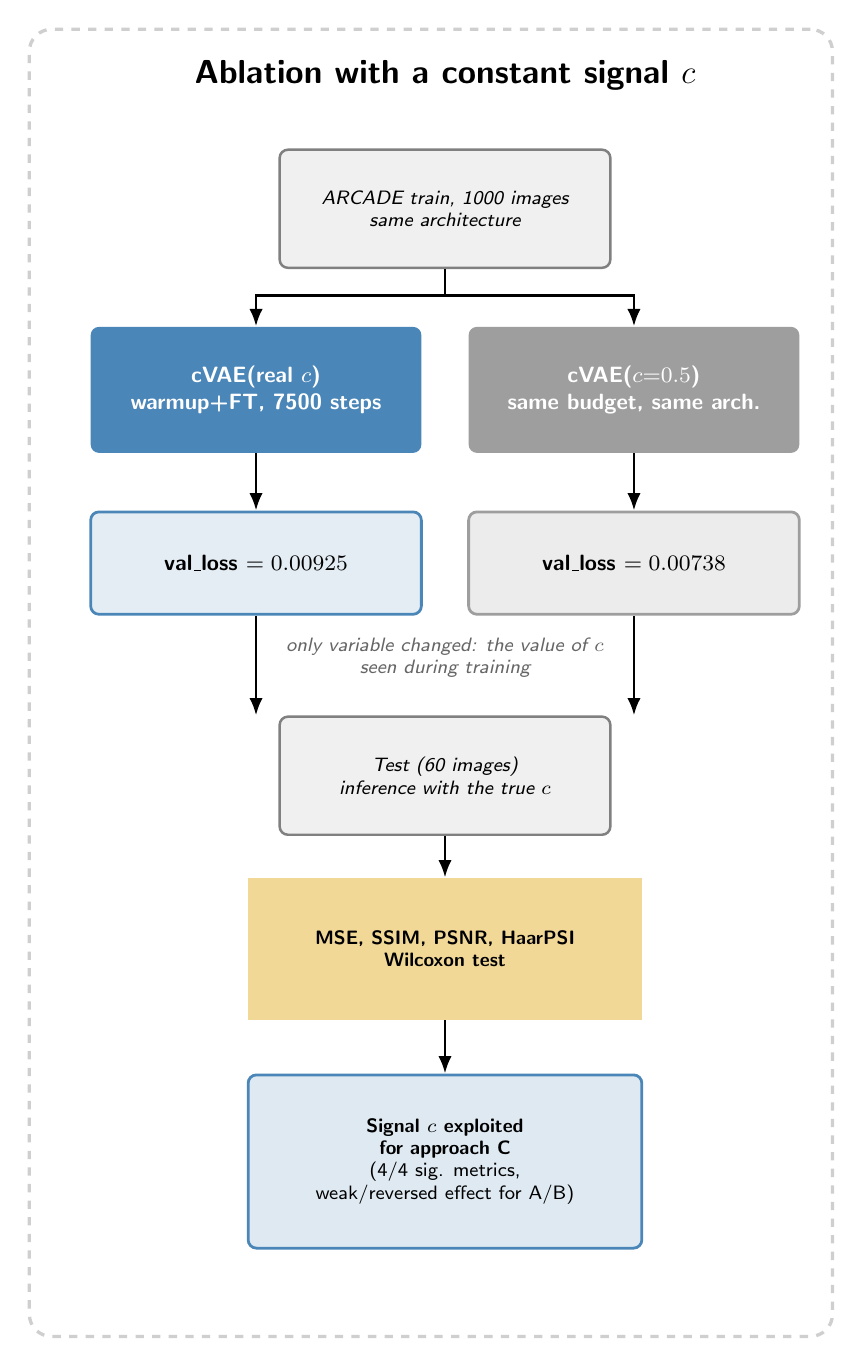
\begin{tikzpicture}[x=1cm,y=1cm]

\node[panel,minimum width=10.2cm,minimum height=16.6cm,anchor=north west] at (-.3,17.5){};

\node[title] at (5.0,16.9) {Ablation with a constant signal $c$};

\node[data] (data) at (5.0,15.2) {ARCADE train, 1000 images\\same architecture};

\node[model]      (creal)  at (2.6,12.9) {cVAE(real $c$)\\warmup+FT, 7500 steps};
\node[constmodel] (cconst) at (7.4,12.9) {cVAE($c{=}0.5$)\\same budget, same arch.};

\draw[arrow] (data.south) -- (5.0,14.1) -- (2.6,14.1) -- (creal.north);
\draw[arrow] (data.south) -- (5.0,14.1) -- (7.4,14.1) -- (cconst.north);

\node[ckpt,draw=medBlue,fill=medBlue!15]     (creal_ckpt)  at (2.6,10.7) {val\_loss $=0.00925$};
\node[ckpt,draw=constGray,fill=constGray!20] (cconst_ckpt) at (7.4,10.7) {val\_loss $=0.00738$};

\draw[arrow] (creal.south)  -- (creal_ckpt.north);
\draw[arrow] (cconst.south) -- (cconst_ckpt.north);

\node[font=\sffamily\scriptsize\itshape,text=black!60,align=center] at (5.0,9.5)
  {only variable changed: the value of $c$\\seen during training};

\node[data] (testset) at (5.0,8.0) {Test (60 images)\\inference with the true $c$};

\draw[arrow] (creal_ckpt.south)  -- (testset.north -| creal_ckpt.south);
\draw[arrow] (cconst_ckpt.south) -- (testset.north -| cconst_ckpt.south);

\node[metricbox,fill=loss1] (metrics) at (5.0,5.8)
  {MSE, SSIM, PSNR, HaarPSI\\Wilcoxon test};

\draw[arrow] (testset.south) -- (metrics.north);

\node[merge] (concl) at (5.0,3.1)
  {Signal $c$ exploited\\for approach C\\{\scriptsize\mdseries (4/4 sig. metrics,}\\{\scriptsize\mdseries weak/reversed effect for A/B)}};

\draw[arrow] (metrics.south) -- (concl.north);

\end{tikzpicture}
\end{document}
